%! TeX root = ../phd-thesis.tex
%! Author = davidedomini

%----------------------------------------------------------------------------------------
\chapter{Frameworks}
\label{chap:frameworks}
\minitoc
%----------------------------------------------------------------------------------------



%=============================================================================
\section{Phyelds}
\label{sec:phyelds}
%=============================================================================

The work presented in this thesis required aggregate programs 
 to interact directly with machine-learning models, training procedures, 
 and multi-agent environments. 
% 
However, 
 the principal \gls{AC} implementations target Java, Scala, or C++, 
 whereas contemporary machine-learning workflows are predominantly developed in Python. 
% 
Using these frameworks would therefore require a cross-language layer around 
 model parameters, tensors, datasets, and simulation environments, 
 complicating both development and prototyping.

Phyelds was developed to remove this barrier by providing 
 a native Python implementation of \gls{AC}~\cite{DBLP:conf/coordination/AguzziDFV26}.
%  
It is not a new calculus: 
 it implements the execution model introduced in the previous sections 
 through an API designed around Python's imperative and object-oriented idioms.
%
This choice allows aggregate coordination to be embedded in ordinary Python
 applications and combined with libraries such as PyTorch and TensorFlow without
 moving data or control across language boundaries. 
% 
The same design also makes the framework suitable for interactive development, education, 
 and integration with Python-based robotics and multi-agent simulation software.

Phyelds was guided by three design goals. 
%
First, 
 the user-facing API should look and behave like conventional Python rather 
 than expose a functional syntax borrowed from another language. 
% 
Second, 
 the implementation should remain lightweight and modular, 
 so that the same core can support notebooks, native simulation, external simulators, 
 and physical deployments. 
% 
Third, 
 aggregate  values should remain ordinary Python values whenever possible, 
 allowing coordination functions to manipulate numbers, collections, model parameters,
 and tensors through their existing interfaces.

\begin{figure}[t]
  \centering
  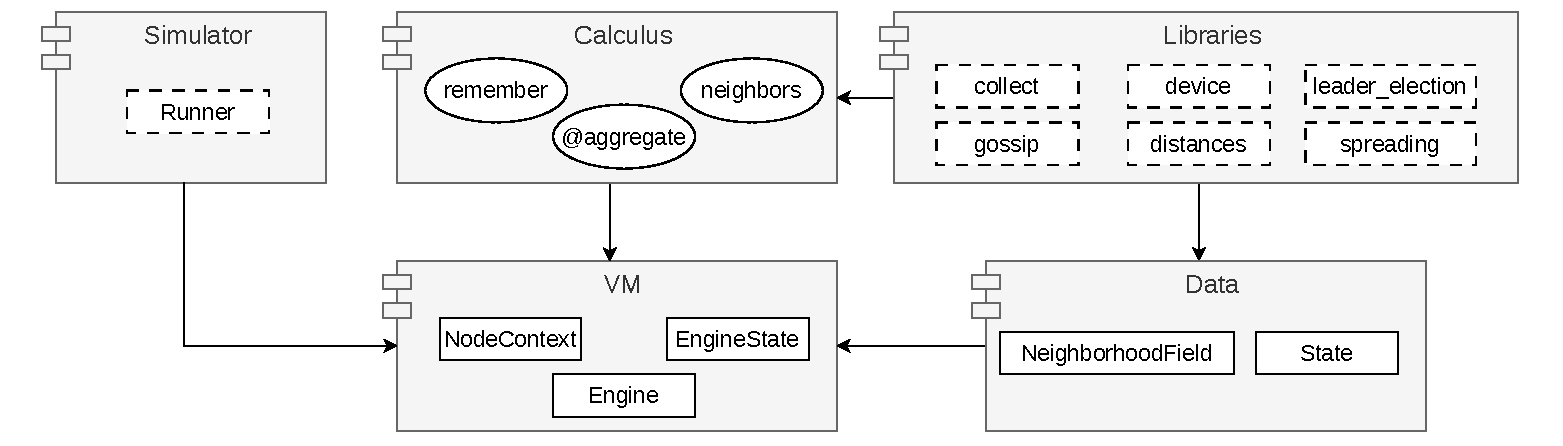
\includegraphics[width=\textwidth]{figures/ch03/phyelds.drawio.pdf}
  \caption{Modular architecture of Phyelds. The virtual machine and data
  modules implement execution and field representation; the calculus exposes
  Pythonic constructs; libraries provide reusable coordination blocks; and the
  simulator supplies execution environments and integration points.}
  \label{fig:phyelds-architecture}
\end{figure}

\subsection{Execution architecture.}
The implementation is organized into five modules, 
 shown conceptually in~\Cref{fig:phyelds-architecture}. 
% 
The \emph{VM} module manages an aggregate round, 
 including the current device context, incoming neighbor messages, persistent state, 
 and alignment paths. 
% 
Its central class is \texttt{Engine}, 
 which exposes a three-stage lifecycle. 
%
Before a round,
 \texttt{setup} installs the device identifier, sensor and time information, 
 messages received from neighbors, and the state produced by the previous round. 
% 
The application then invokes the aggregate function as an ordinary Python function. 
%
Finally, 
 \texttt{cooldown} returns the updated state and the messages to transmit, 
 and resets the engine for the next execution.

This separation keeps the aggregate program independent from the component that schedules it. 
%
A native simulator, 
 an external environment, or a physical device runtime only needs to construct the context, 
 invoke the program, and deliver its outputs. 
% 


\subsection{Pythonic calculus constructs.}
The \emph{Calculus} module maps the constructs discussed 
 in~\Cref{sec:field-calculus} to Python. 
% 
Its entry point is the \texttt{@aggregate} decorator, 
 which marks a function as part of an aggregate program. 
% 
The decorator wraps each invocation with calls that enter 
 and leave a named execution scope. 
% 
These scopes extend the current alignment path, 
 allowing the engine to distinguish state and messages produced 
 by different functions or different occurrences of the same operator.

State evolution is exposed through \texttt{remember}. 
%
Instead of receiving an update function as in a functional \texttt{rep}, 
 \texttt{remember(initial)} returns the current value together with a setter. 
% 
The program can read and update the state imperatively, 
 following a pattern similar to state management in Python application frameworks.
% 
Internally, 
 the value is represented by a \texttt{State} proxy that records both the stored object 
 and the alignment path of the corresponding call.

Neighbor interaction is exposed through \texttt{neighbors(value)}. 
%
The call shares \texttt{value} and returns a \texttt{NeighborhoodField}, 
 which internally maps device identifiers to the latest aligned values received from those devices. 
% 
The implementation hides this mapping behind a regular Python object. 
%
It supports pointwise arithmetic, field combination, 
 and explicit aggregation through \texttt{foldhood}, 
 with convenience methods for common operations such as minimum and maximum. 
% 
When a \texttt{State} object is passed to \texttt{neighbors}, transmission is lazy:
 the value is exported only when it has changed, avoiding repeated exchange of unchanged state.

\Cref{lst:phyelds-api} illustrates the resulting style. 
%
The program uses a normal Python conditional, 
 updates persistent state through a setter, 
 and operates on neighbor values as a Python object. 
% 
No explicit engine or message management appears in the application code.

\begin{lstlisting}[language=Python,float=t,
  caption={Pythonic state, branching, and neighbor interaction in Phyelds.},
  label={lst:phyelds-api}]
@aggregate
def active_counter():
    set_counter, counter = remember(0)

    if sense("active"):
        counter += 1
        set_counter(counter)

    neighbor_counters = neighbors(counter)
    return neighbor_counters.max()
\end{lstlisting}

The use of an ordinary \texttt{if} requires special handling.
%
In \gls{FC},
 branching also partitions the alignment domain,
 whereas a Python conditional normally affects only local control flow.
%
Phyelds reconciles the two semantics transparently: when an aggregate function
 is decorated, its \texttt{if} statements are wrapped in distinct alignment
 contexts, so devices taking different branches do not exchange values within
 those branches.
%
This transformation is invisible to the developer,
 who writes plain Python conditionals and relies on the engine
 to maintain correct alignment across the collective.

\subsection{Libraries and execution environments.}
The \emph{Library} module builds reusable coordination functions 
 on top of the Pythonic calculus. 
% 
Its submodules separate device access, time, distance metrics, spreading, 
collection, gossip, and leader election. 
%
For example,
 \texttt{distance\_to}, \texttt{broadcast}, and \texttt{cast\_from} 
 implement information spreading; 
 \texttt{collect\_with}, \texttt{count\_nodes}, and \texttt{sum\_values} 
 implement aggregation toward a source; and
 \texttt{elect\_leaders} supports decentralized spatial partitioning. 
% 
These functions accept and return Python objects, 
 so the same coordination paths can carry sensor readings, collections, 
 or machine-learning model parameters.

The \emph{Simulator} module provides a compact execution environment 
 without coupling the calculus to a particular deployment. 
% 
A \texttt{Node} stores a device identifier, position, and sensor data; 
 an \texttt{Environment} manages nodes and computes their neighborhoods; 
 and a discrete-event \texttt{Simulator} schedules aggregate rounds. 
% 
Neighborhood policies are pluggable and may describe communication 
 by radius, nearest neighbors, full connectivity, or a user-defined relation. 
% 
Monitors receive execution callbacks for inspection and visualization. 
%
External systems can instead provide a runner and an environment adapter; 
 the VMAS integration follows this pattern, keeping the aggregate program independent 
 from the underlying multi-agent simulator.

For this thesis,
 Phyelds provides the implementation layer connecting field-based coordination
 with Python-native learning code.
%
Local training, model aggregation, inference, and policy computation remain ordinary
 Python operations, while \texttt{remember}, \texttt{neighbors}, and the coordination
 library determine how their state and outputs evolve across the collective.
%
This separation is used throughout the contribution chapters:
 in~\Cref{chap:selforg-fl}, field-based operators organize self-adaptive federation
 structures around local federated learning procedures;
 in~\Cref{chap:scalable-rl}, coordination determines what each agent observes
 and how collective state is summarized for decentralized policy learning;
 and in~\Cref{chap:tasksplacement}, the same abstractions support decentralized
 application placement decisions across the edge--cloud continuum.



%=============================================================================
\section{ProFed: Benchmarking Proximity-Based Federated Learning}
\label{sec:selforgfl-benchmarking}
%=============================================================================

\subsection{Motivation}

The evaluation of federated learning algorithms relies heavily 
 on benchmark suites that provide common datasets, partitioning strategies, 
 and evaluation protocols.
%
Existing frameworks cover several complementary aspects of this process.
%
For example, 
 FedScale~\cite{DBLP:conf/icml/LaiDSLZMC22} supports large-scale experiments 
 on realistic datasets while accounting for system heterogeneity 
 and client resource constraints.
%
Similarly, 
 LEAF~\cite{DBLP:journals/corr/abs-1812-01097} 
  promotes reproducible evaluation through standardized datasets, metrics, 
  and reference implementations, including measurements of model performance and training costs.
%
Other benchmarks provide configurable environments for comparing federated learning algorithms 
 on established datasets under different client-level
 partitions~\cite{DBLP:journals/corr/abs-2007-13518,DBLP:journals/corr/abs-2007-14390}.

These frameworks provide valuable support for the evaluation 
 of general-purpose federated learning methods.
%
However, 
 their data-partitioning procedures typically abstract away 
 the spatial organization of the clients.
%
Data are assigned directly to individual devices without representing the fact that, 
 in many collective adaptive systems, nearby devices experience similar conditions 
 and consequently observe correlated data distributions.
%
Examples include vehicles operating within the same urban district, 
 sensors deployed in a shared physical environment, 
 and devices located within the same industrial site.

This limitation is particularly relevant to the methods introduced in this chapter.
%
All the algorithms presented in this chapter explicitly exploit 
 the relation between spatial proximity and data similarity, 
 assuming that data are relatively homogeneous within a region 
 but heterogeneous across different regions.
%
Evaluating such algorithms through conventional client-level partitions 
 does not capture this structure and makes it difficult to systematically investigate how
 regional heterogeneity affects federation formation and learning performance.

ProFed~\cite{DBLP:journals/jors/DominiIALV26} addresses this gap 
 by providing a standardized benchmark  for generating region-aware federated learning scenarios.
%
Rather than distributing data independently among clients, 
 it first partitions a dataset across spatial regions according to a configurable degree of heterogeneity
 and subsequently distributes each regional partition among the devices located within that region.
%
This enables reproducible evaluation of proximity-based federated learning algorithms 
 under controlled spatial data distributions and facilitates their
 comparison across datasets, partitioning strategies, and levels of regional skewness.

\subsection{Implementation}

ProFed implementation is based on PyTorch~\cite{DBLP:conf/asplos/AnselYHGJVBBBBC24} 
 and TorchVision~\cite{TorchVision}, 
 as it has been specifically designed to facilitate and 
 standardize research experiments within the scenario described above. 
%
ProFed provides an API to partition the supported datasets and 
 to generate experimental scenarios that follow the proposed system model. 
% 
In particular, 
 given the number of regions and the number of devices per region, 
 it enables the creation of region-aware data partitions such that 
 devices belonging to the same region receive datasets sampled from 
 the same underlying data distribution. 
%
This design allows the benchmark to reproduce realistic proximity-based non-IID scenarios, 
 where data are homogeneous within regions and heterogeneous across regions, 
 as illustrated in~\Cref{fig:spatial-heterogeneity}.
%
The following paragraphs detail the implemented methods to synthesize skewed datasets, 
 the supported datasets and the API of the benchmark.



\paragraph{Data Distribution.} The supported partitioning methods were selected 
 by reviewing studies in the literature on non-IID 
 Federated Learning and identifying the most commonly used ones.
%
Several works employ the \emph{Dirichlet} distribution for data partitioning. 
%
This approach results in each party having instances of most labels, 
 although the distribution is highly imbalanced, 
 with some labels being underrepresented and others heavily overrepresented.
%
The degree of skewness can be adjusted using the concentration parameter 
 $\alpha$, where lower values yield more skewed distributions.
%
In the literature, $\alpha$ values typically range from 0.1 to 1.0, 
 with $\alpha=0.5$ commonly used for moderate heterogeneity.
%
An example of this distribution, for $5$ subregions and the MNIST dataset (with $10$ classes), 
 is represented in~\Cref{fig:dirichlet}.
%
The second data distribution considered is \emph{hard} partitioning,
 where each party has access to only a subset of labels.
%
This creates a significantly more skewed distribution, 
 making it considerably more challenging for learning algorithm stability.
%
An example of this distribution is represented in~\Cref{fig:hard}.
%
ProFed enables fine-grained control over the data distribution, allowing either 
 balanced label subsets across regions or customizable cardinality per subregion.
%
For comparative analysis, ProFed also implements an IID split as a baseline distribution (\Cref{fig:iid}).
%
While existing approaches typically apply these partitioning methods 
 directly at the device level (e.g.,~\cite{DBLP:journals/corr/abs-2302-02949,DBLP:conf/nips/LinKSJ20}), 
 ProFed introduces an intermediate layer of regional clustering.
% 
ProFed first distributes data heterogeneously among subregions and 
 then splits them homogeneously among devices within the same subregion,
 thereby creating clustered heterogeneity---see~\Cref{fig:spatial-heterogeneity}.
%
To support extensibility, ProFed enables custom partitioning 
 based on a user-specified distribution matrix. 
%
This distribution is represented as an $N \times M$ matrix 
 where $N$ is the number of labels and $M$ is the number of subregions. 
%
Each cell $(i,j)$ indicates the proportion of instances with label $i$ 
 assigned to subregion $j$.

\begin{figure}
\centering
\begin{subfigure}{0.3\textwidth}
    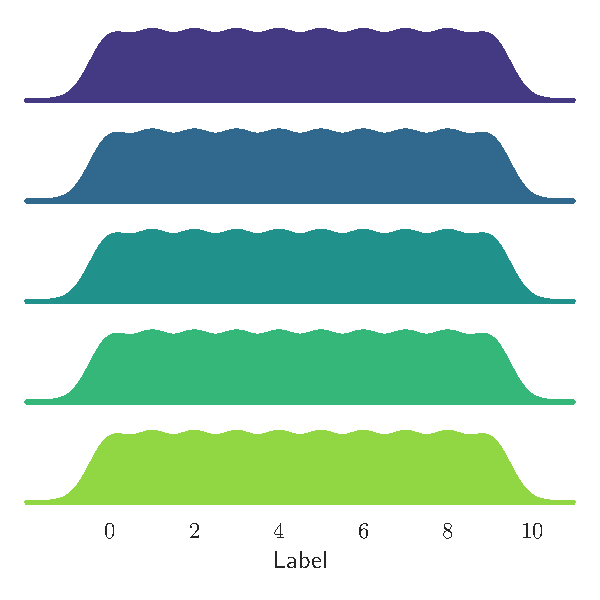
\includegraphics[width=\textwidth]{figures/ch07/profed/IID.pdf}
    \caption{IID}
    \label{fig:iid}
    \end{subfigure}
\begin{subfigure}{0.3\textwidth}
    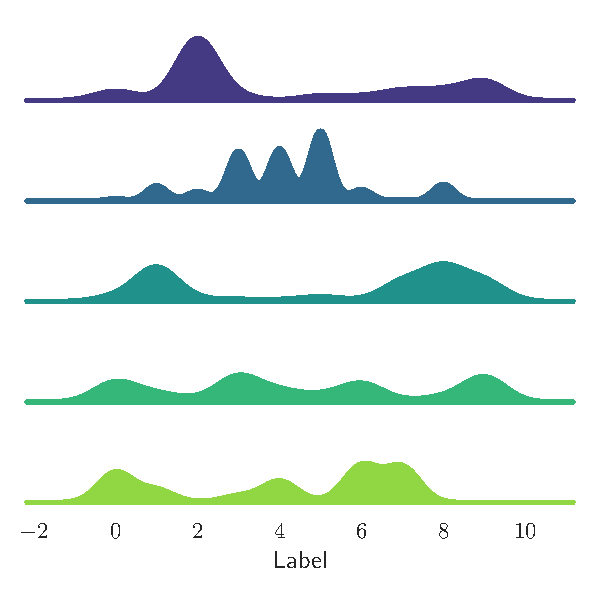
\includegraphics[width=\textwidth]{figures/ch07/profed/Dirichlet.pdf}
    \caption{Dirichlet}
    \label{fig:dirichlet}
    \end{subfigure}
\begin{subfigure}{0.3\textwidth}
    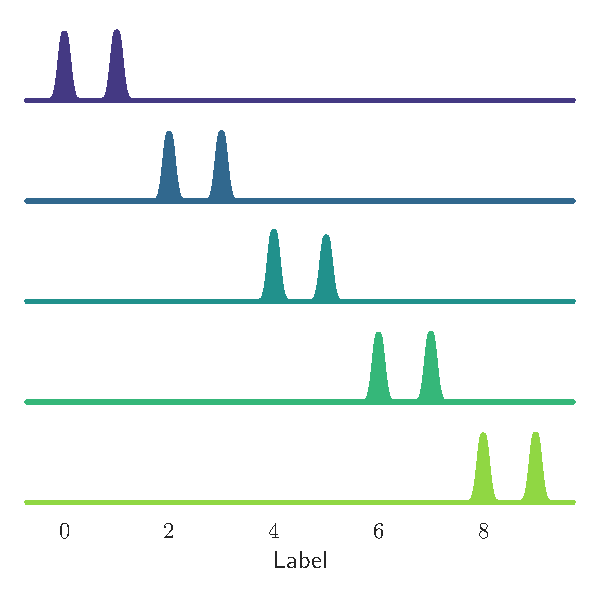
\includegraphics[width=\textwidth]{figures/ch07/profed/Hard.pdf}
    \caption{Hard}
    \label{fig:hard}
\end{subfigure}
\caption{ 
    Data distribution patterns across 5 subregions: (a) IID data, (b) Dirichlet (Non-IID), and (c) Hard (Highly Non-IID).
    Each color represents a different subregion.
 }
\label{fig:skewness}
\end{figure}


\paragraph{Supported Datasets.}
ProFed supports various TorchVision datasets widely used in computer vision research 
 (details in~\Cref{tab:datasets}). 
%
MNIST~\cite{lecun2010mnist} is included as a baseline: 
 grayscale $28 \times 28$ pixel images of handwritten digits across 10 classes.
%
ProFed extends this with Fashion MNIST~\cite{DBLP:journals/corr/abs-1708-07747} (clothing items, 10 classes) 
 and Extended MNIST~\cite{DBLP:journals/corr/CohenATS17} (EMNIST, Latin alphabet letters, 27 classes). 
% 
For color images, ProFed includes CIFAR10 and CIFAR100 with 32x32 RGB images. 
%
CIFAR10 has 10 classes while CIFAR100 has 100, offering greater complexity. 
%
Beyond classification tasks, ProFed incorporates the UTKFace dataset \cite{DBLP:conf/cvpr/ZhangSQ17}, 
 containing over 23,000 face images based on 200 $\times$ 200 pixel RGB images, 
 for age regression tasks.  
%
All classification datasets maintain balanced class distributions 
 (e.g., CIFAR10 provides 6,000 training instances per class).

\begin{table}
    \centering
    \caption{
        Summary of the characteristics of the datasets included in the benchmark.
        The first five datasets are designed for classification tasks, 
         with target values corresponding to discrete classes.
        In contrast, the last dataset is used for a regression task, 
        where the target values span a continuous range.
        }
    \label{tab:datasets}
    \begin{tabular}{lrrrr}
    \toprule
    \textbf{Dataset} & \textbf{Training Size} & \textbf{Test Size} & \textbf{Features} & \textbf{Targets} \\ 
    \midrule
    MNIST           & 60,000 & 10,000 & 784  & 10  \\ 
    Fashion MNIST   & 60,000 & 10,000 & 784  & 10 \\ 
    EMNIST  & 124,800 & 20,800 & 784  & 27 \\ 
    CIFAR-10       & 50,000 & 10,000 & 3,072 & 10 \\ 
    CIFAR-100      & 50,000 & 10,000 & 3,072 & 100 \\ 
    UTKFace       & 20150 & 3557 & 120000 & $[1;116]$\\
    \bottomrule
    \end{tabular}
\end{table}

\paragraph{Benchmark API.} 
ProFed has been designed with usability and ergonomics in mind. 
%
To achieve this, its API provides all the necessary methods 
 to manage the referenced use case seamlessly---an example is provided in Listing~\ref{lst:api-example}.
%
First, ProFed allows users to download the selected dataset directly 
 and automatically generate training and validation subsets.
%
Second, and most important, given a dataset and a predefined number of subregions,
 it enables users to distribute data among subregions following the
 specified distribution strategy.
%
Finally, once the data distribution among subregions is established, 
 ProFed facilitates the creation of datasets for individual devices. 
%
Each device-specific dataset is represented as an instance of the \texttt{Subset} class from PyTorch, 
 ensuring full compatibility with existing learning algorithms. % based on it.

%\noindent\begin{minipage}{\columnwidth}
\lstdefinestyle{proFedStyle}{
    backgroundcolor=\color{gray!5},
    frame=single,
    rulecolor=\color{black!20},
    frameround=tttt,
    framesep=8pt,
    xleftmargin=10pt,
    xrightmargin=10pt,
    basicstyle=\ttfamily\scriptsize,
    breaklines=true,
    captionpos=b,
    %numbers=left,
    numberstyle=\tiny\color{gray!70},
    language=python,
    keywordstyle=\color{blue!80!black},
    commentstyle=\color{green!50!black},
    stringstyle=\color{red!70!black},
    showstringspaces=false,
    tabsize=4,
    breakatwhitespace=false,
    breakindent=20pt,
}

\begin{figure*}
\begin{lstlisting}[style=proFedStyle, caption={An example of how ProFed is used to partition the EMNIST dataset among devices}, label={lst:api-example}]
from ProFed.partitioner import Environment, Region, download_dataset, split_train_validation, partition_to_subregions

mapping_devices_area = distribute_nodes_spatially(devices, number_subregions)

train_data, test_data = download_dataset('EMNIST')
train_data, validation_data = split_train_validation(train_data, 0.8)

environment = partition_to_subregions(train_data, validation_data, 'Hard', number_subregions, seed)

mapping = {}

for region_id, devices in mapping_devices_area.items():
    mapping_devices_data = environment.from_subregion_to_devices(
		region_id, 
		len(devices))
    for device_index, data in mapping_devices_data.items():
        device_id = devices[device_index]
        mapping[device_id] = data
\end{lstlisting}
\end{figure*}

\subsection{Quality Control}
\paragraph{Experimental Setup}
To evaluate ProFed's effectiveness and usability, 
 experiments were conducted on the supported datasets with three
 state-of-the-art algorithms: 
 FedAvg~\cite{DBLP:conf/aistats/McMahanMRHA17}, 
 FedProx~\cite{DBLP:conf/mlsys/LiSZSTS20}, and 
 Scaffold~\cite{DBLP:conf/icml/KarimireddyKMRS20}.
%
Data were synthetically partitioned using  
 supported methods: IID, Dirichlet ($\alpha=0.5$), and Hard partitioning.
%
Experiments varied the number of subregions $A \in \{3, 6, 9\}$.
%
All implementations utilized PyTorch with consistent hyperparameters across approaches. 
%
A multi-layer perceptron with 128 hidden neurons was
 trained for 30 global rounds. 
% 
Each global round comprised 2 local epochs per device 
 with batch size 32, ADAM optimizer (learning rate $10^{-3}$, 
 weight decay $10^{-4}$).
% 
Experiments were repeated with 5 random seeds for statistical robustness,
 totaling 120 experimental configurations.

All code is publicly available under a permissive license for
 reproducibility purposes\footnote{\url{https://github.com/davidedomini/experiments-2025-jors}}.

\paragraph{Discussion}
Results were systematically collected during training, validation, and testing phases.
A baseline was first established using a homogeneous data distribution (IID) to assess model stability and accuracy. 
%
FedAvg was the only algorithm evaluated under IID conditions, 
 whereas FedProx and Scaffold were not considered in this setting, 
 as they are variants of FedAvg whose distinguishing mechanisms are specifically 
 designed to address non-IID data distributions and therefore provide meaningful 
 differences primarily under data heterogeneity.
%
Under IID conditions, FedAvg demonstrates stable convergence and achieves high accuracy.
% 
This stability is evident in both validation and testing phases.
%
Validation convergence is shown in the first column of \Cref{fig:exp}, 
 where accuracy increases monotonically toward the optimum. 
%
Test stability is demonstrated in \Cref{tab:test}, 
 where the model maintains high accuracy with minimal variance.

The critical impact of data distribution becomes apparent when transitioning 
 from IID to non-IID conditions.
Under heterogeneous data distribution, significant performance degradation occurs. 
% 
All evaluated algorithms fail to handle extreme data skewness effectively, 
 resulting in reduced accuracy and convergence instability. 
%
This degradation is particularly pronounced under hard partitioning. 
%
The bottom row of \Cref{fig:exp} illustrates hard partitioning across nine regions, 
 where validation accuracy drops from $80\%$ (IID) to $50\%$. 
%
Testing results exhibit similar trends. 
%
While FedAvg achieves stable performance above $95\%$ under IID conditions, 
 Dirichlet partitioning introduces substantial instability, 
 evidenced by increased accuracy variance. 
%
Performance decline intensifies under hard partitioning, 
 highlighting fundamental limitations of current federated learning approaches 
 in handling extreme data heterogeneity.
%
These findings indicate that state-of-the-art algorithms inadequately address 
 spatially distributed data challenges, necessitating further research 
 toward more robust solutions.
\begin{table}
    \centering
    \caption{Results on the test set for different algorithms with different partitioning methods.}
    \label{tab:test}
    \begin{tabular}{c|ccc}
    \toprule
    \textbf{Algorithm} & \textbf{IID} & \textbf{Dirichlet} & \textbf{Hard} \\ 
    \midrule
    FedAvg        & 0.95 $\pm$ 0.001 & 0.9 $\pm$ 0.04 & 0.81 $\pm$ 0.01  \\ 
    FedProx       & \ding{55} &  0.886 $\pm$ 0.04 & 0.86 $\pm$ 0.01 \\ 
    Scaffold      & \ding{55} & 0.889 $\pm$ 0.06 &  0.81 $\pm$ 0.01 \\ 
    \bottomrule
    \end{tabular}
\end{table}


\begin{figure*}
    \centering

    % MNIST

    \begin{subfigure}{0.32\textwidth}
        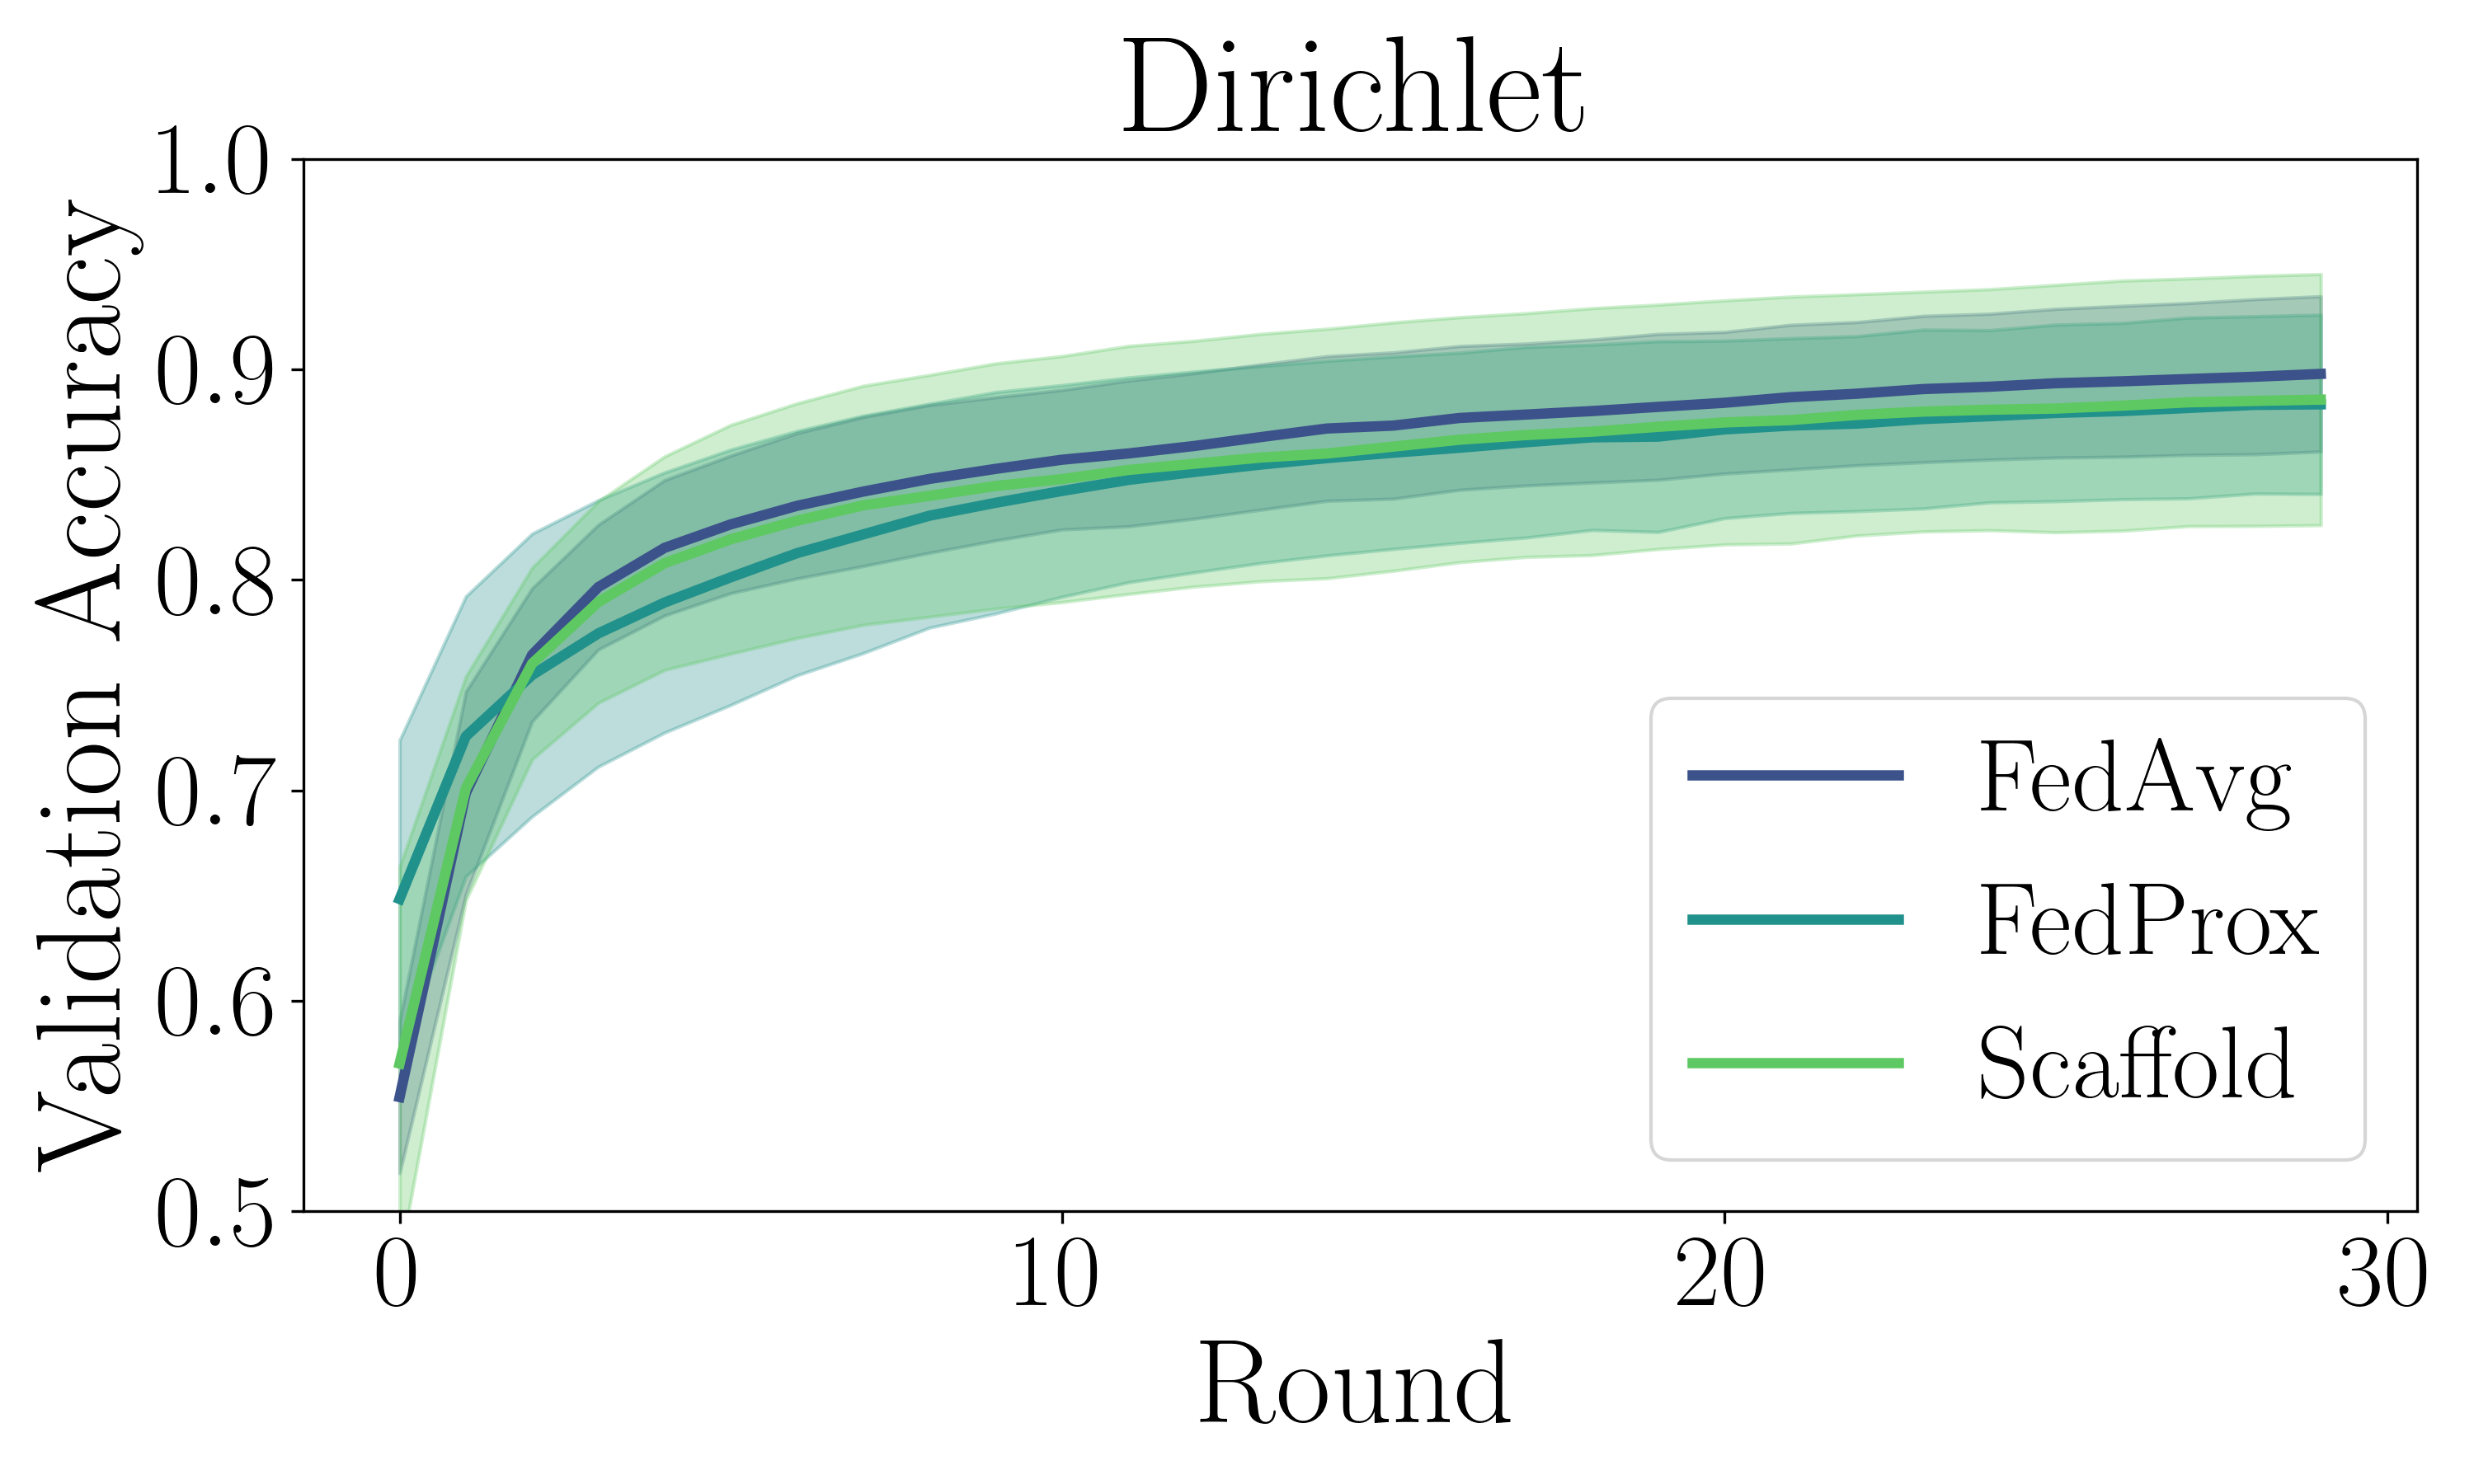
\includegraphics[width=\textwidth]{figures/ch07/profed/charts/ValidationAccuracy_dataset-MNIST_areas-3_partitioning-Dirichlet.png}
        % \caption{TBD}
        % \label{fig:exp-dirichlet}
    \end{subfigure}
    \begin{subfigure}{0.32\textwidth}
        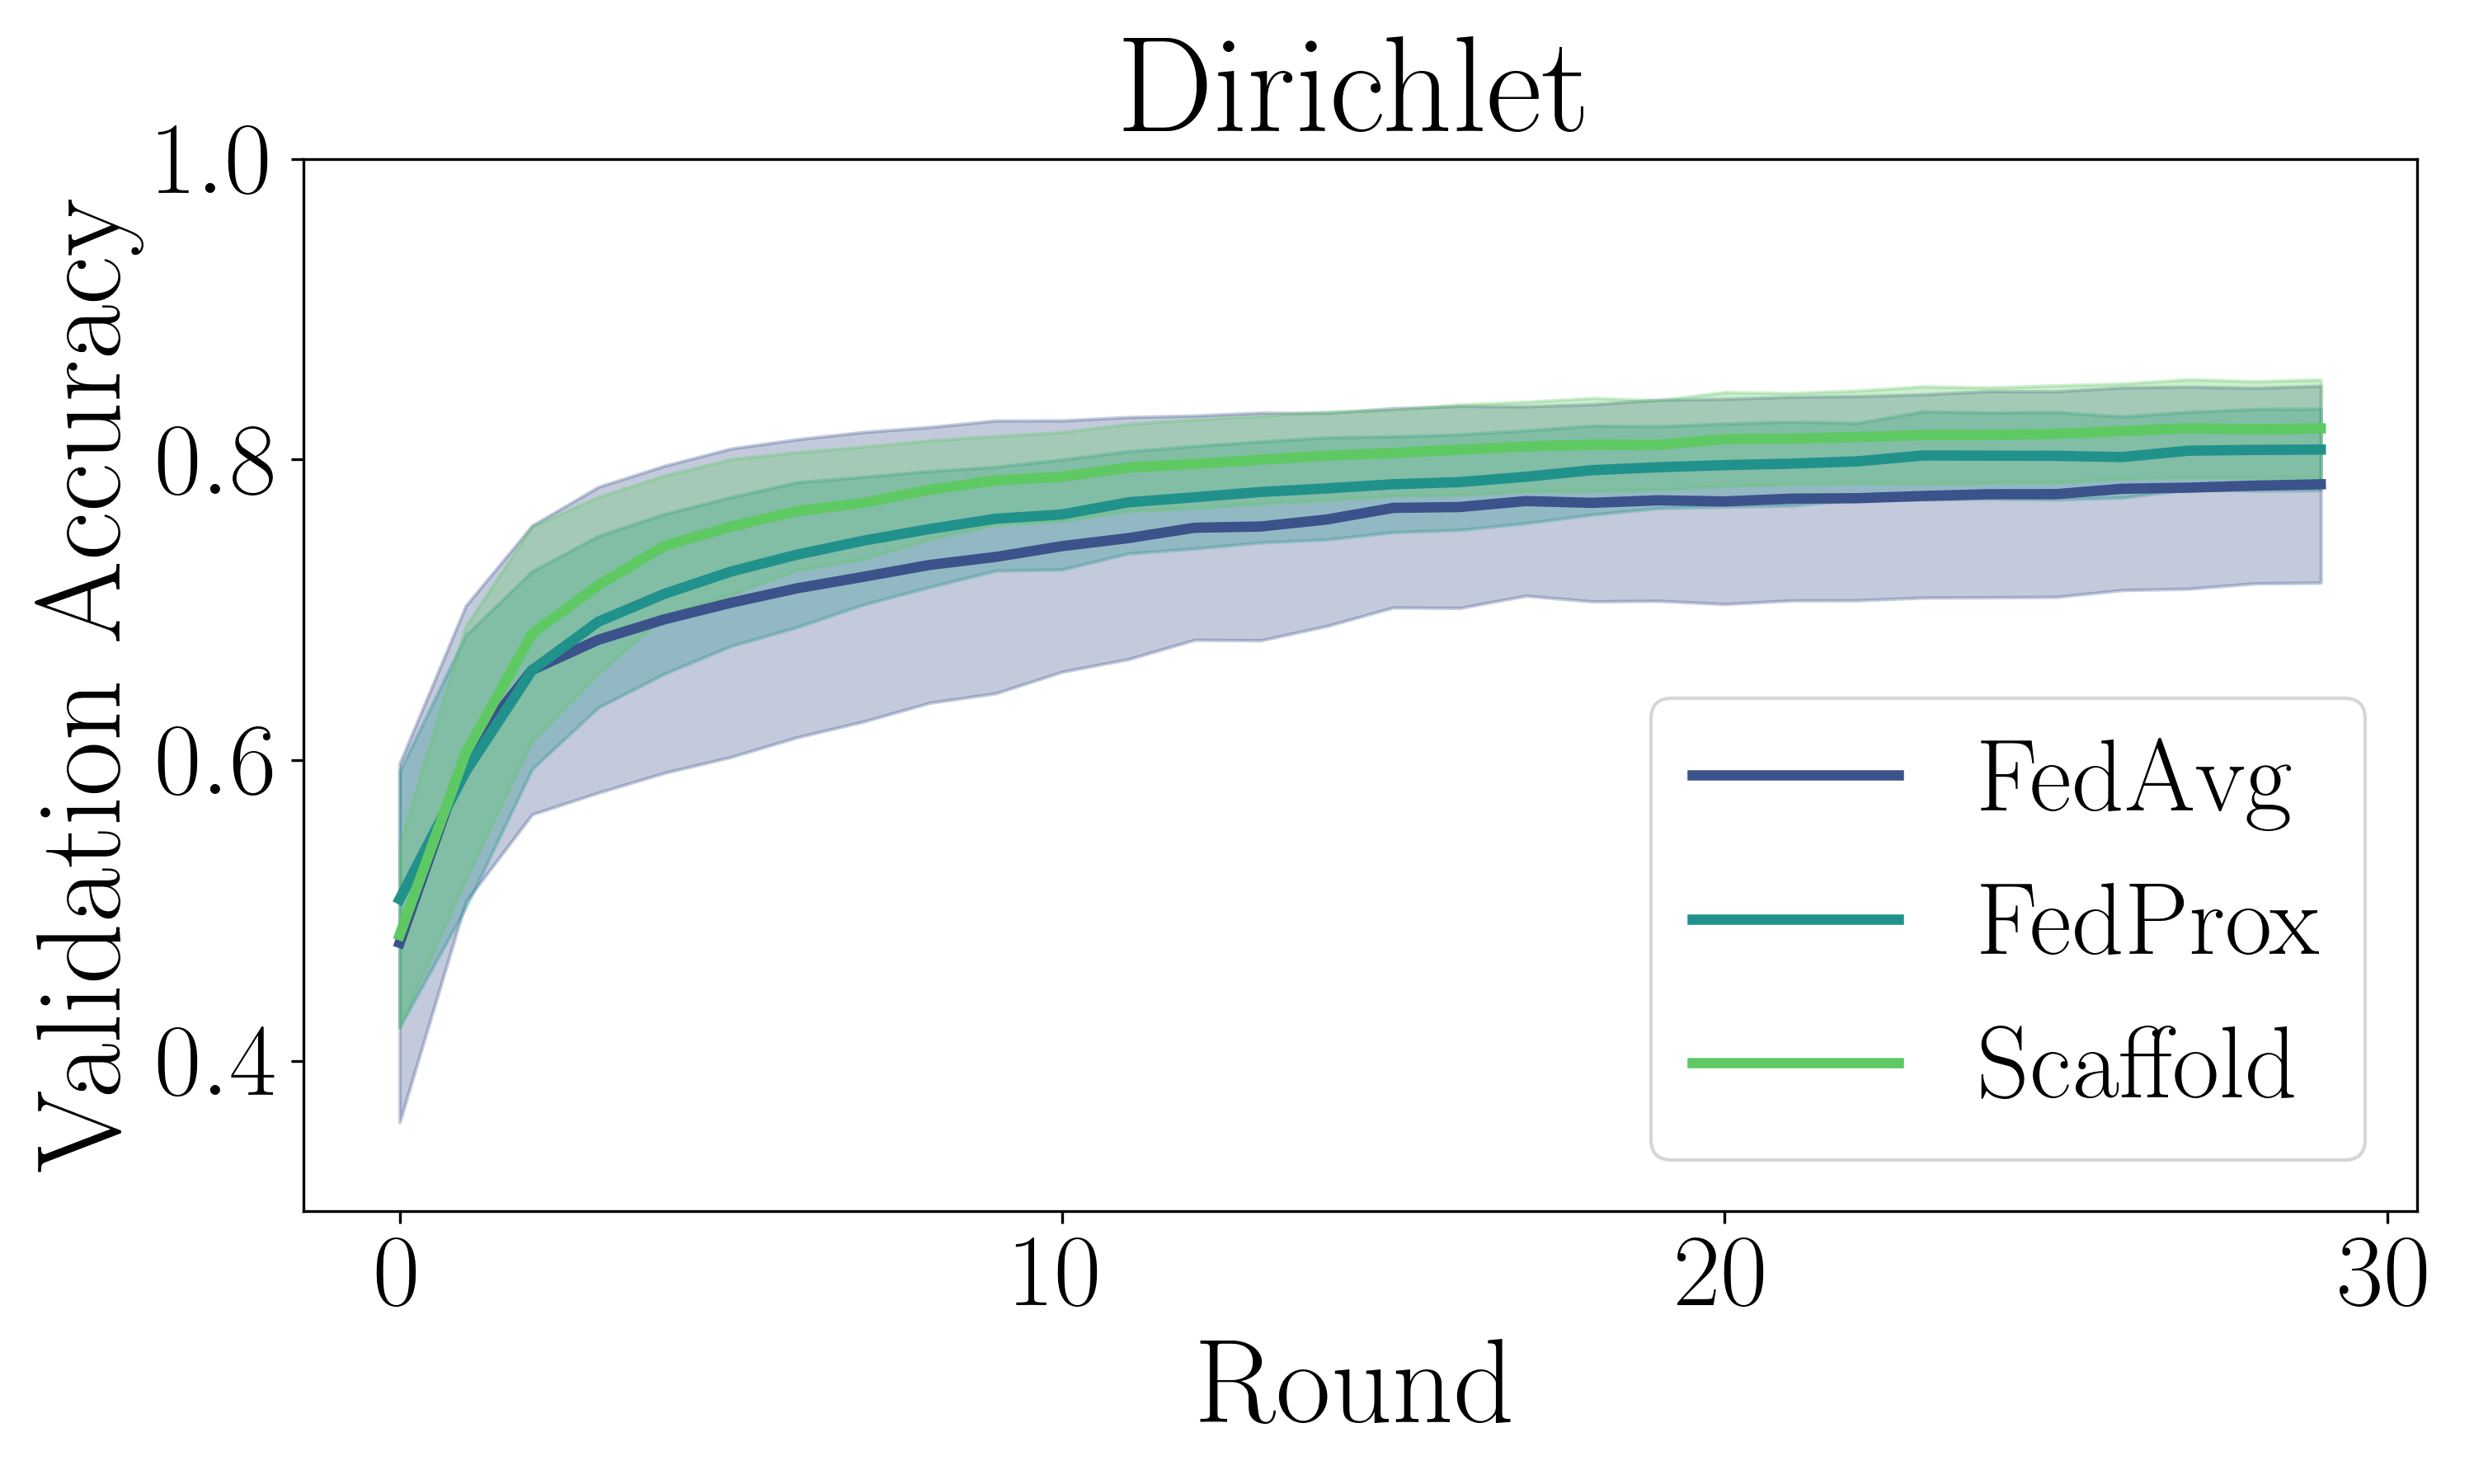
\includegraphics[width=\textwidth]{figures/ch07/profed/charts/ValidationAccuracy_dataset-FashionMNIST_areas-3_partitioning-Dirichlet.png}
        % \caption{TBD}
        % \label{fig:exp-dirichlet}
    \end{subfigure}
    \begin{subfigure}{0.32\textwidth}
        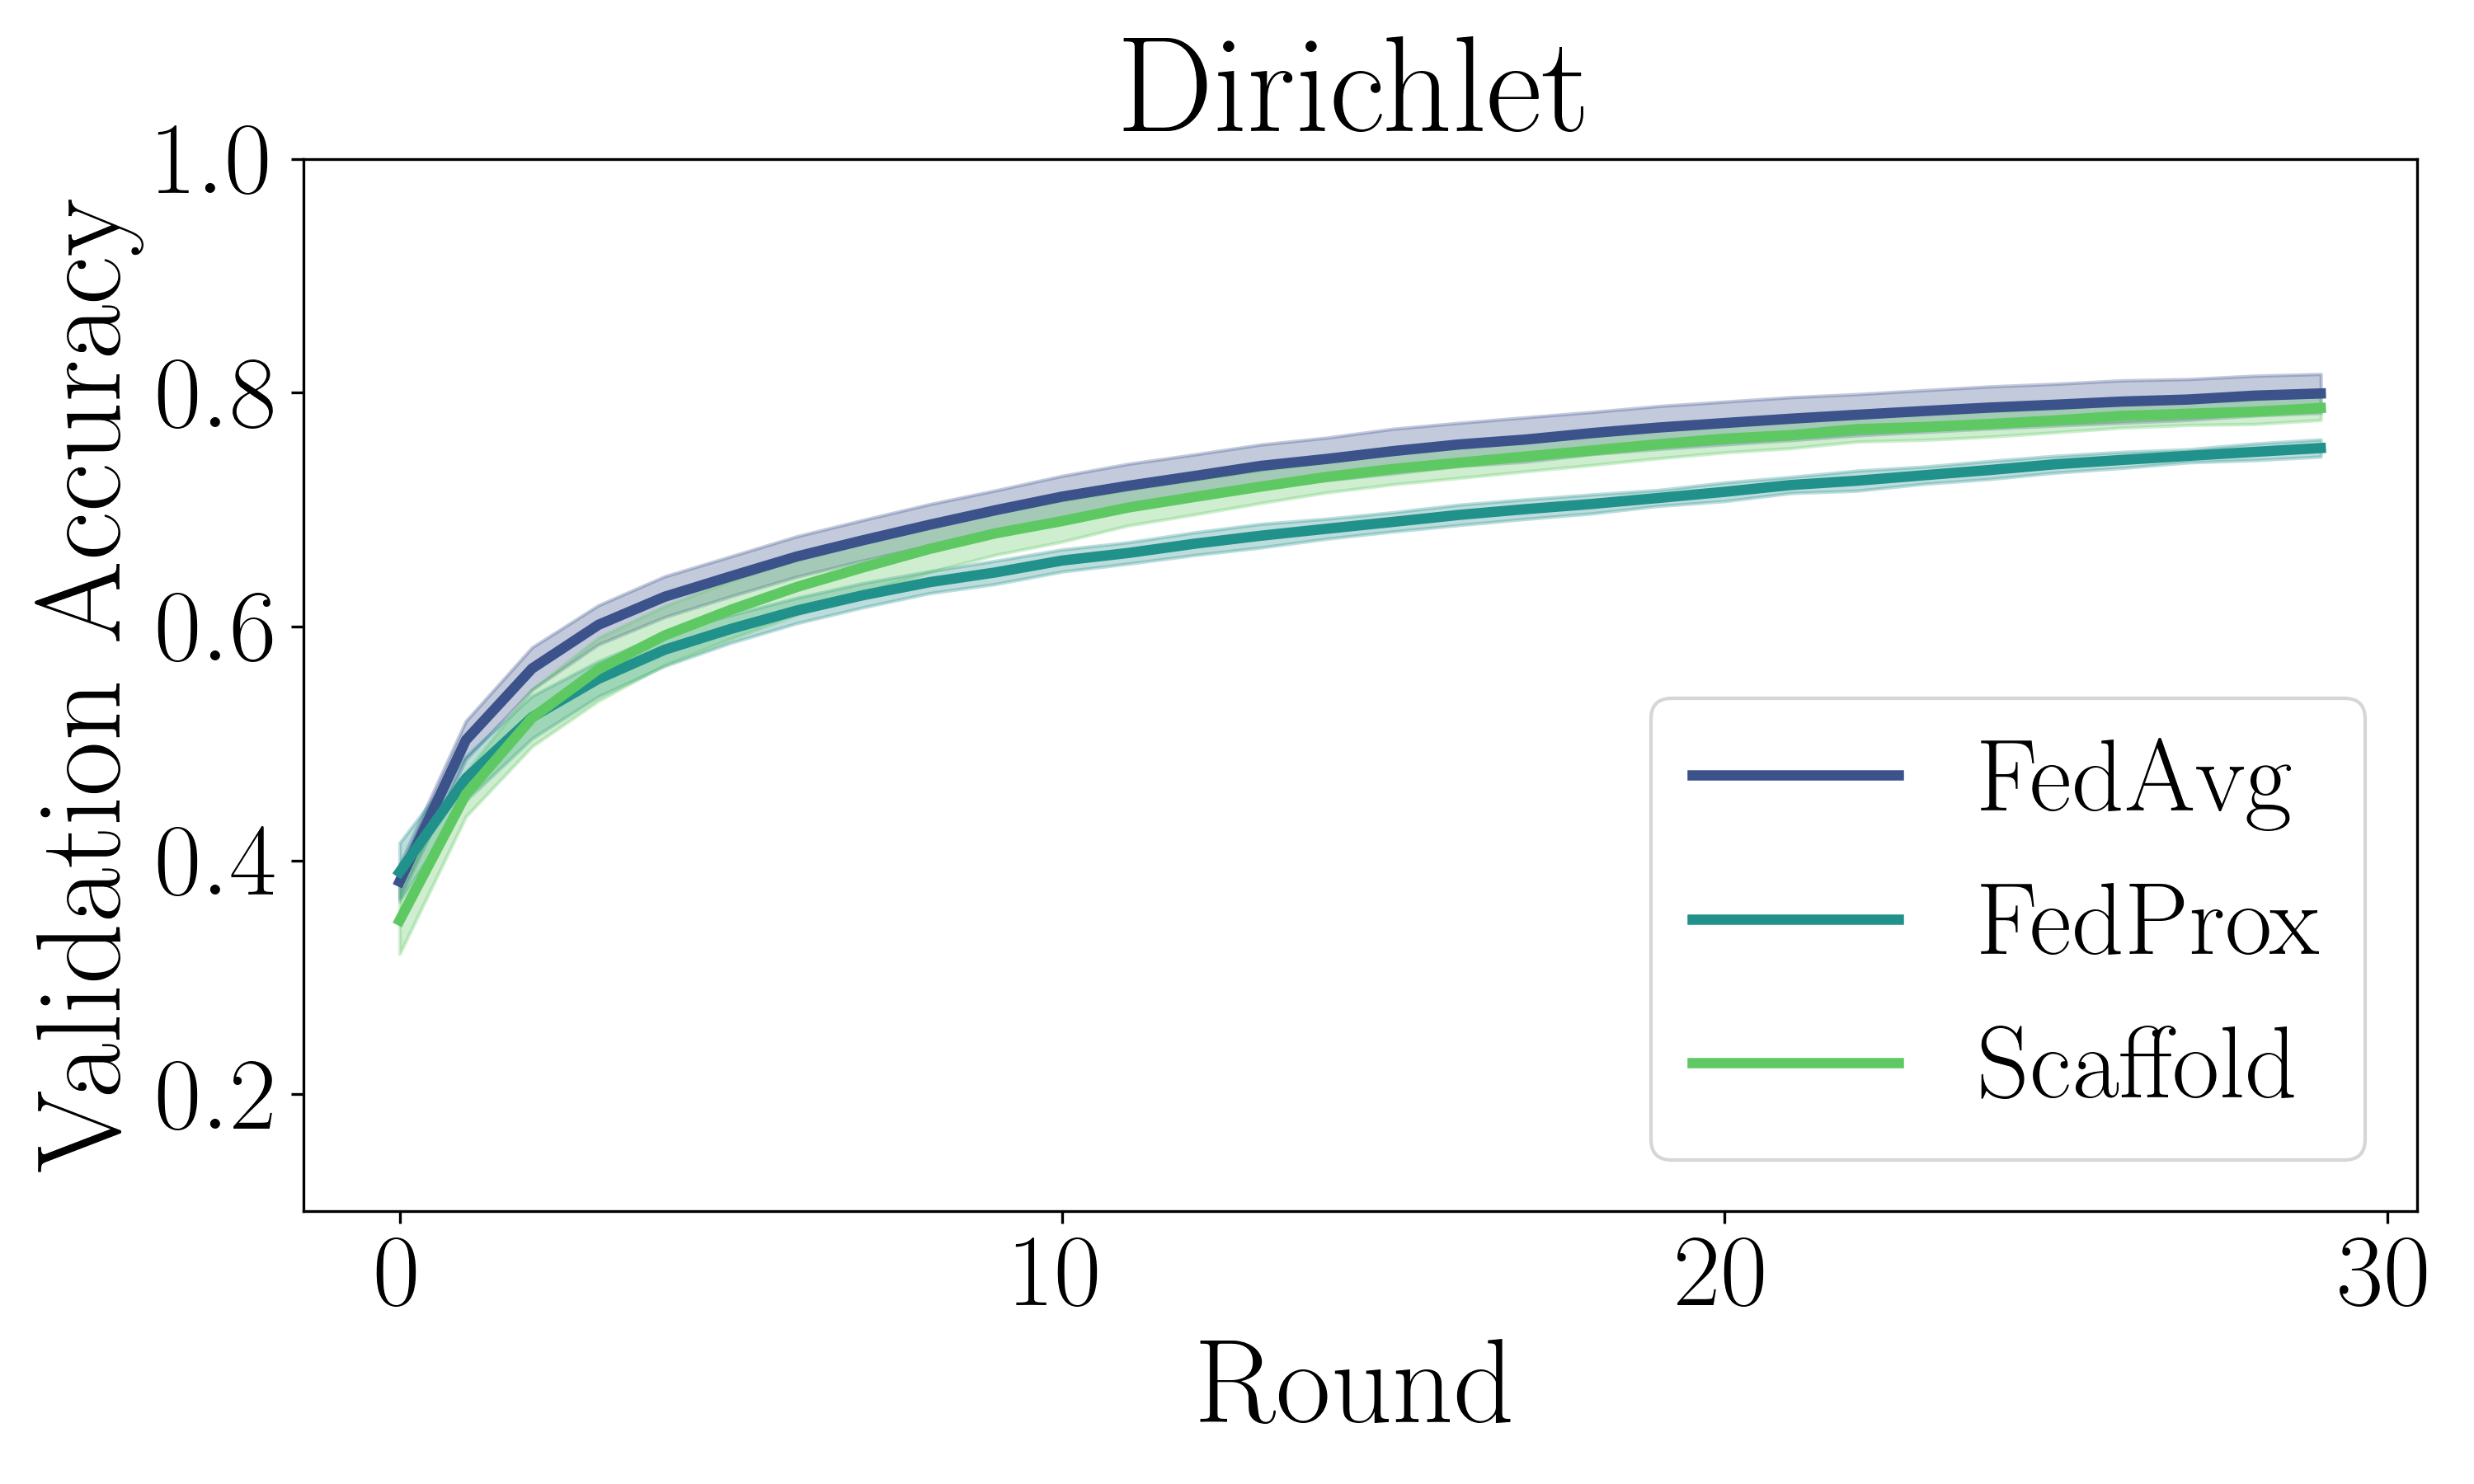
\includegraphics[width=\textwidth]{figures/ch07/profed/charts/ValidationAccuracy_dataset-EMNIST_areas-9_partitioning-Dirichlet.png}
    \end{subfigure}
    \begin{subfigure}{0.32\textwidth}
        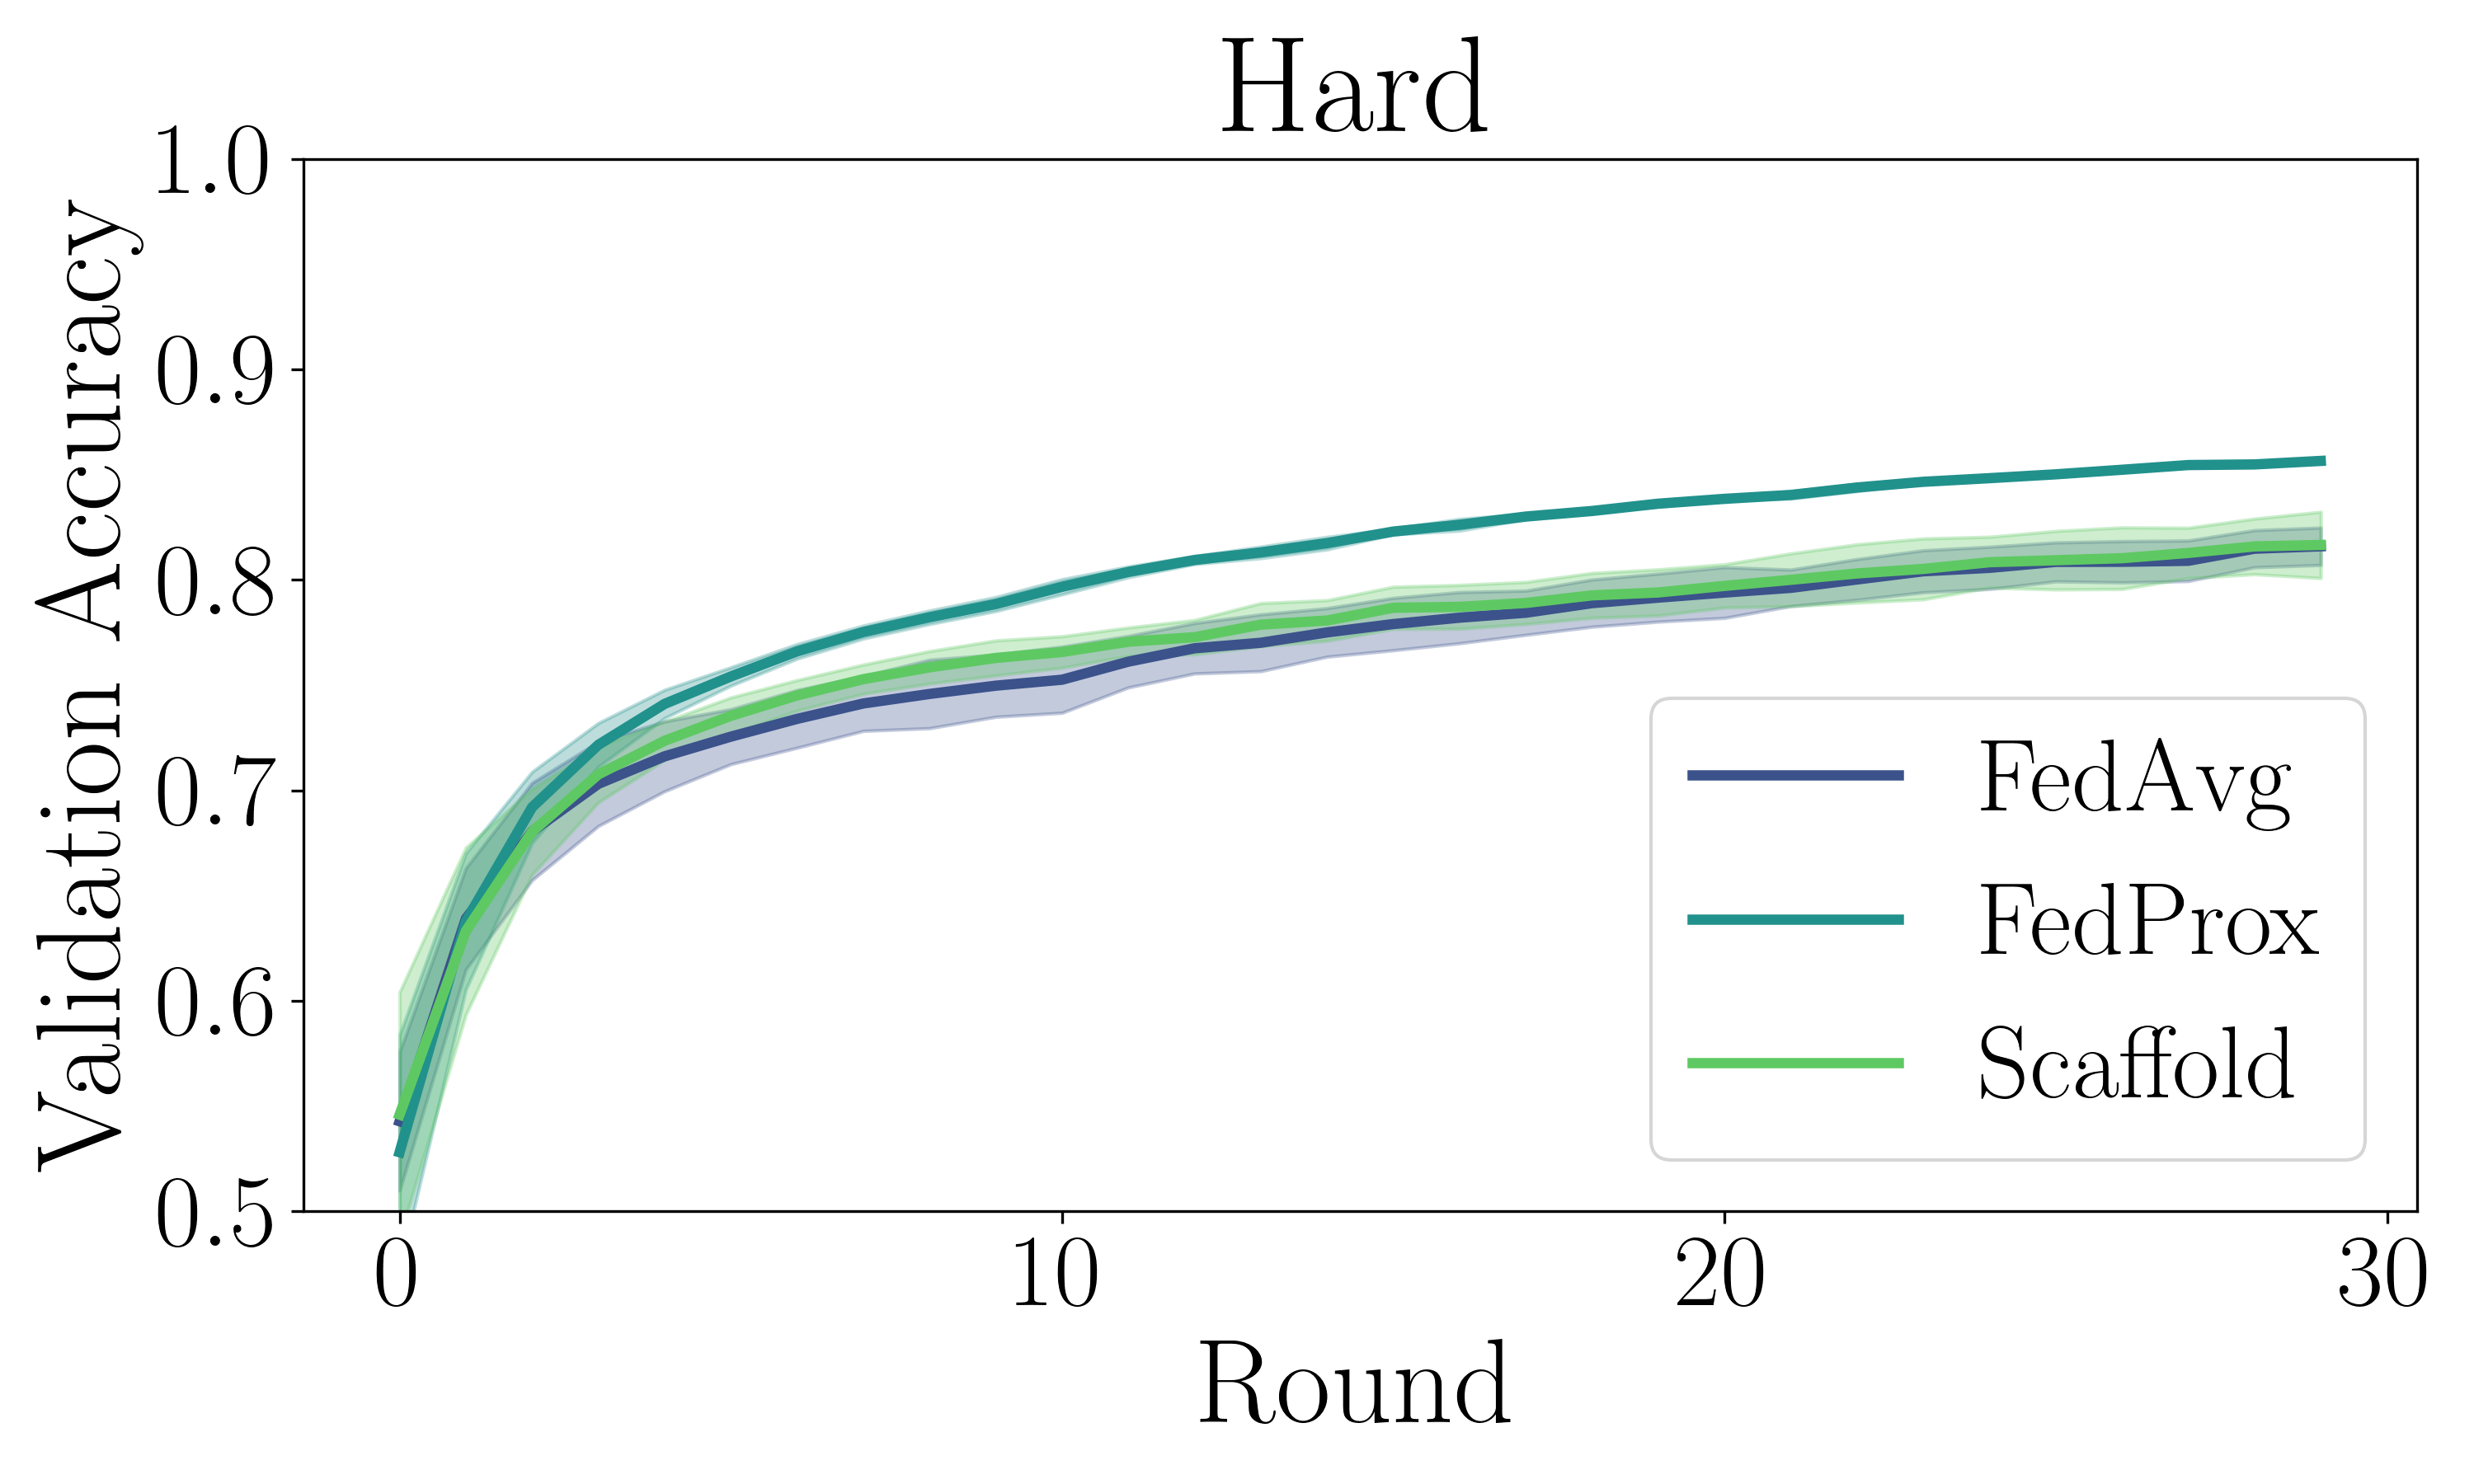
\includegraphics[width=\textwidth]{figures/ch07/profed/charts/ValidationAccuracy_dataset-MNIST_areas-3_partitioning-Hard.png}
        % \caption{TBD.}
        % \label{fig:exp-hard}
    \end{subfigure}
    \begin{subfigure}{0.32\textwidth}
        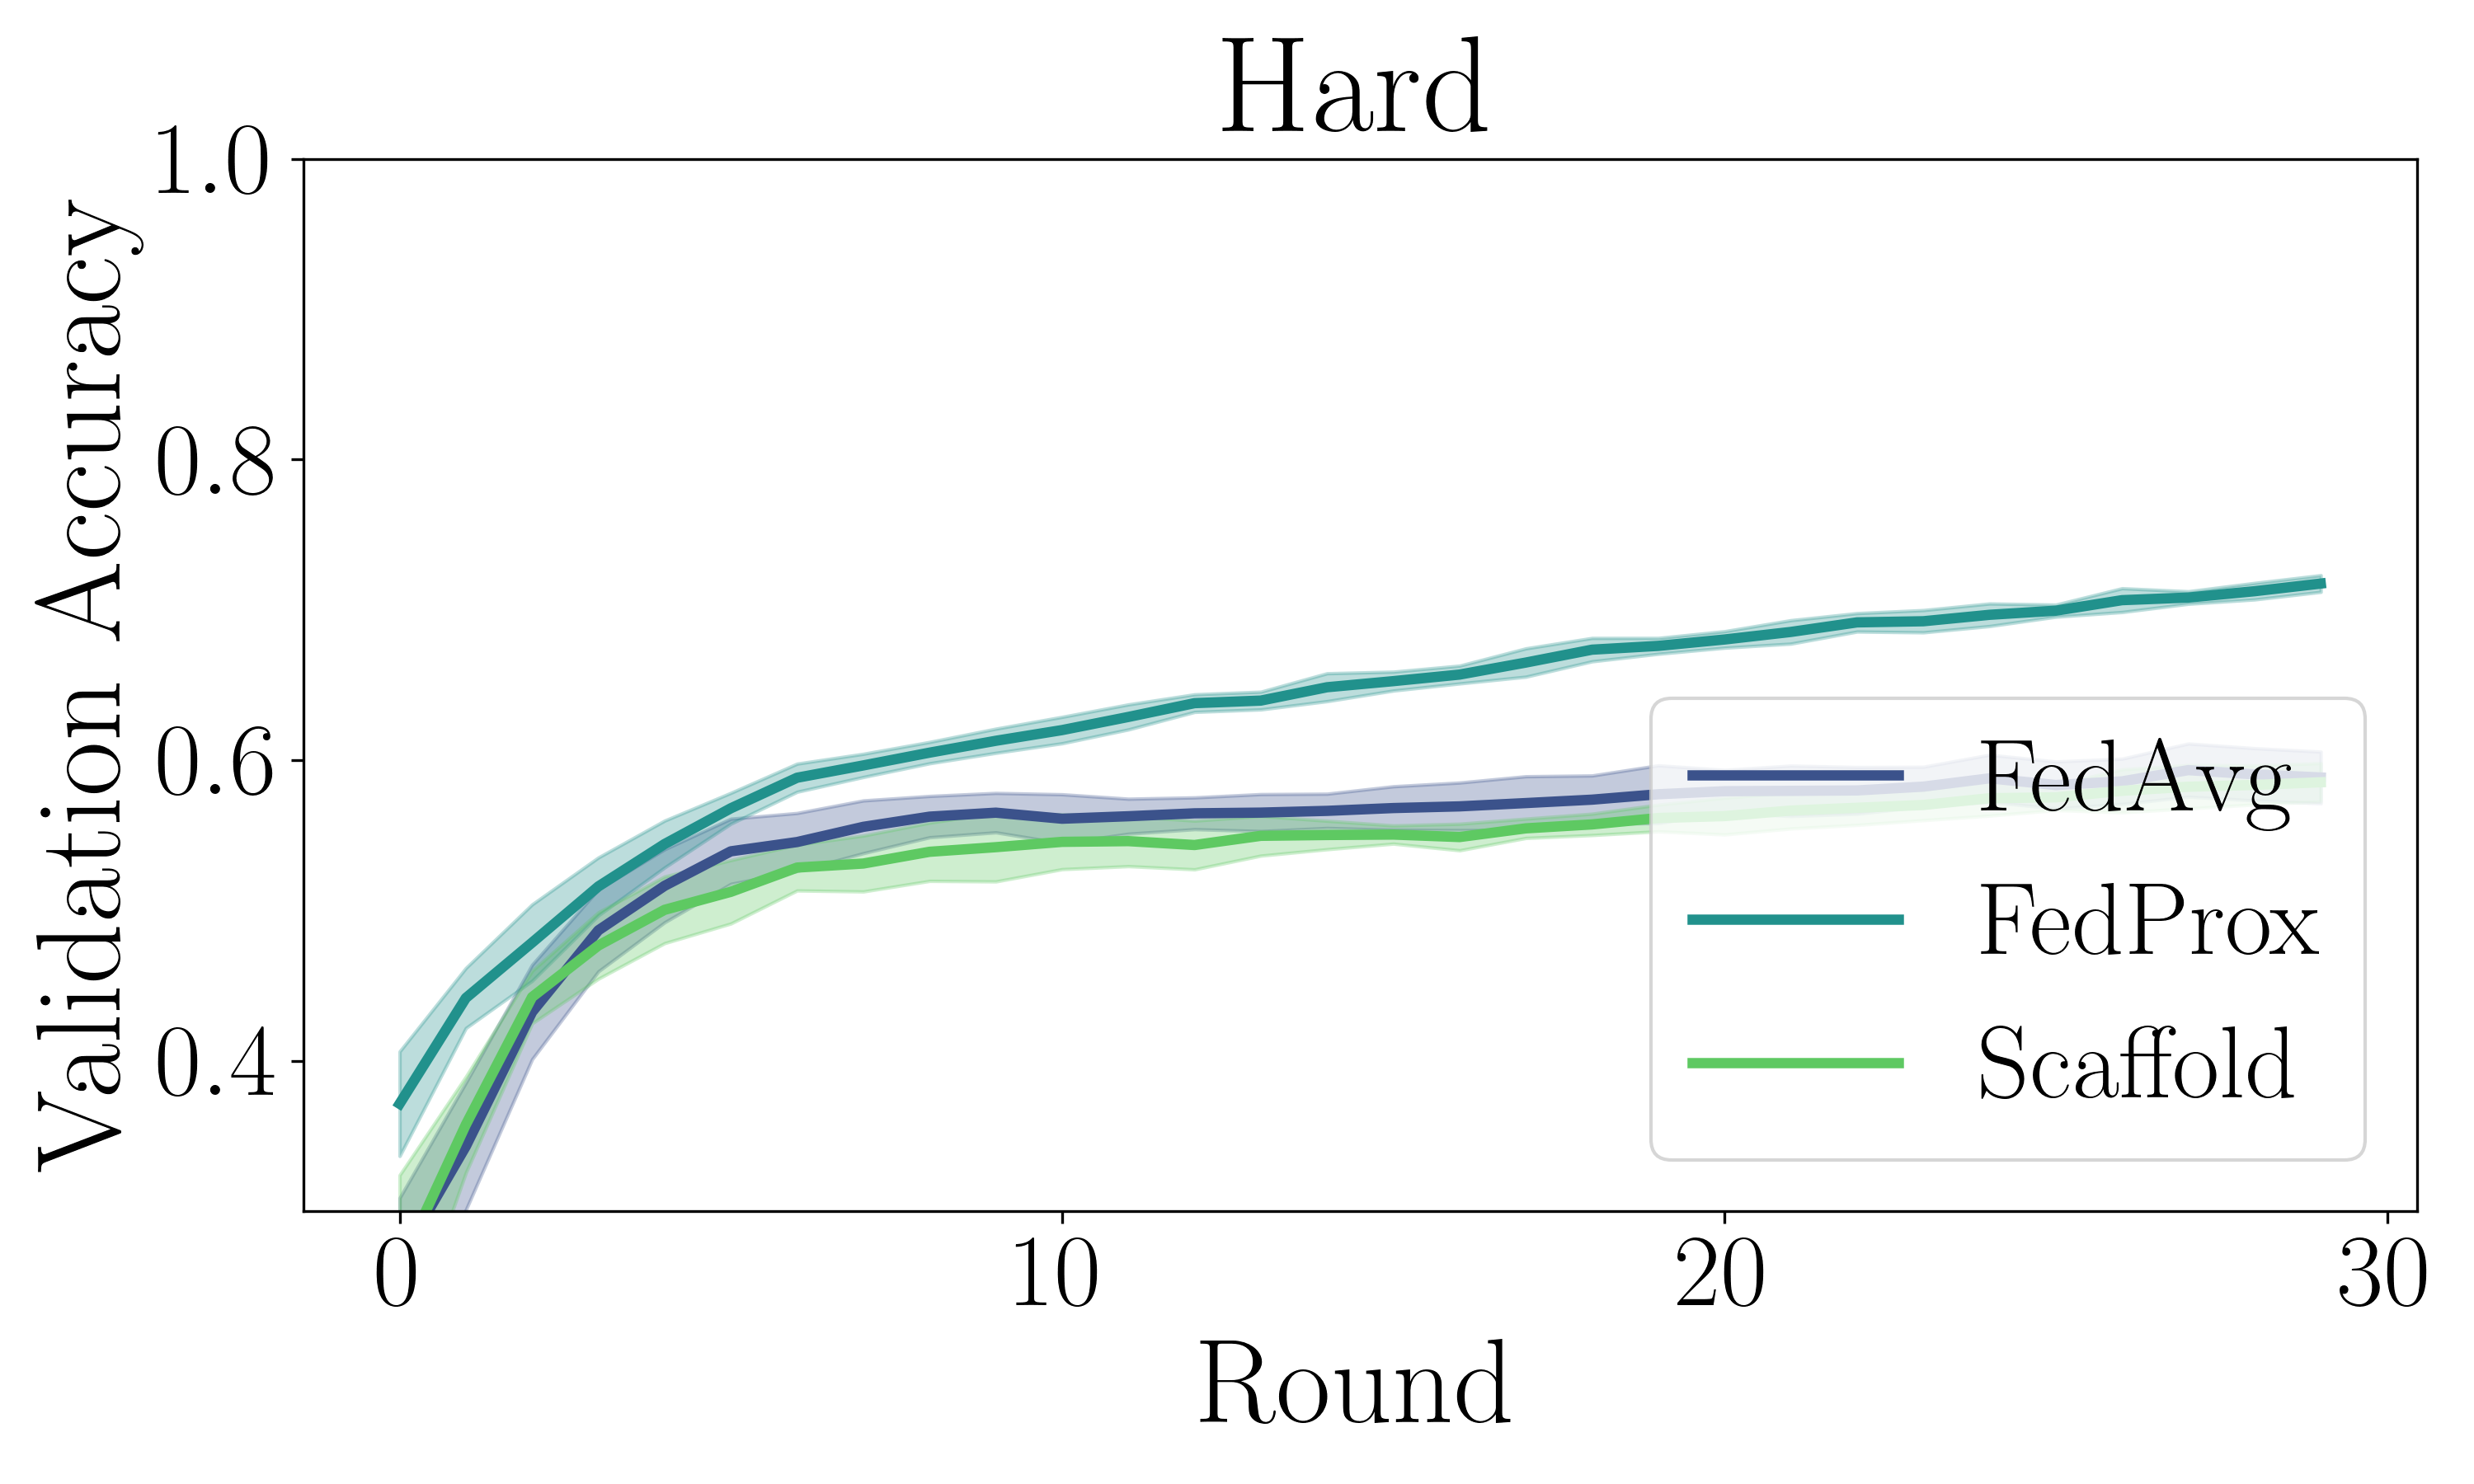
\includegraphics[width=\textwidth]{figures/ch07/profed/charts/ValidationAccuracy_dataset-FashionMNIST_areas-3_partitioning-Hard.png}
        % \caption{TBD.}
        % \label{fig:exp-hard}
    \end{subfigure}
    \begin{subfigure}{0.32\textwidth}
        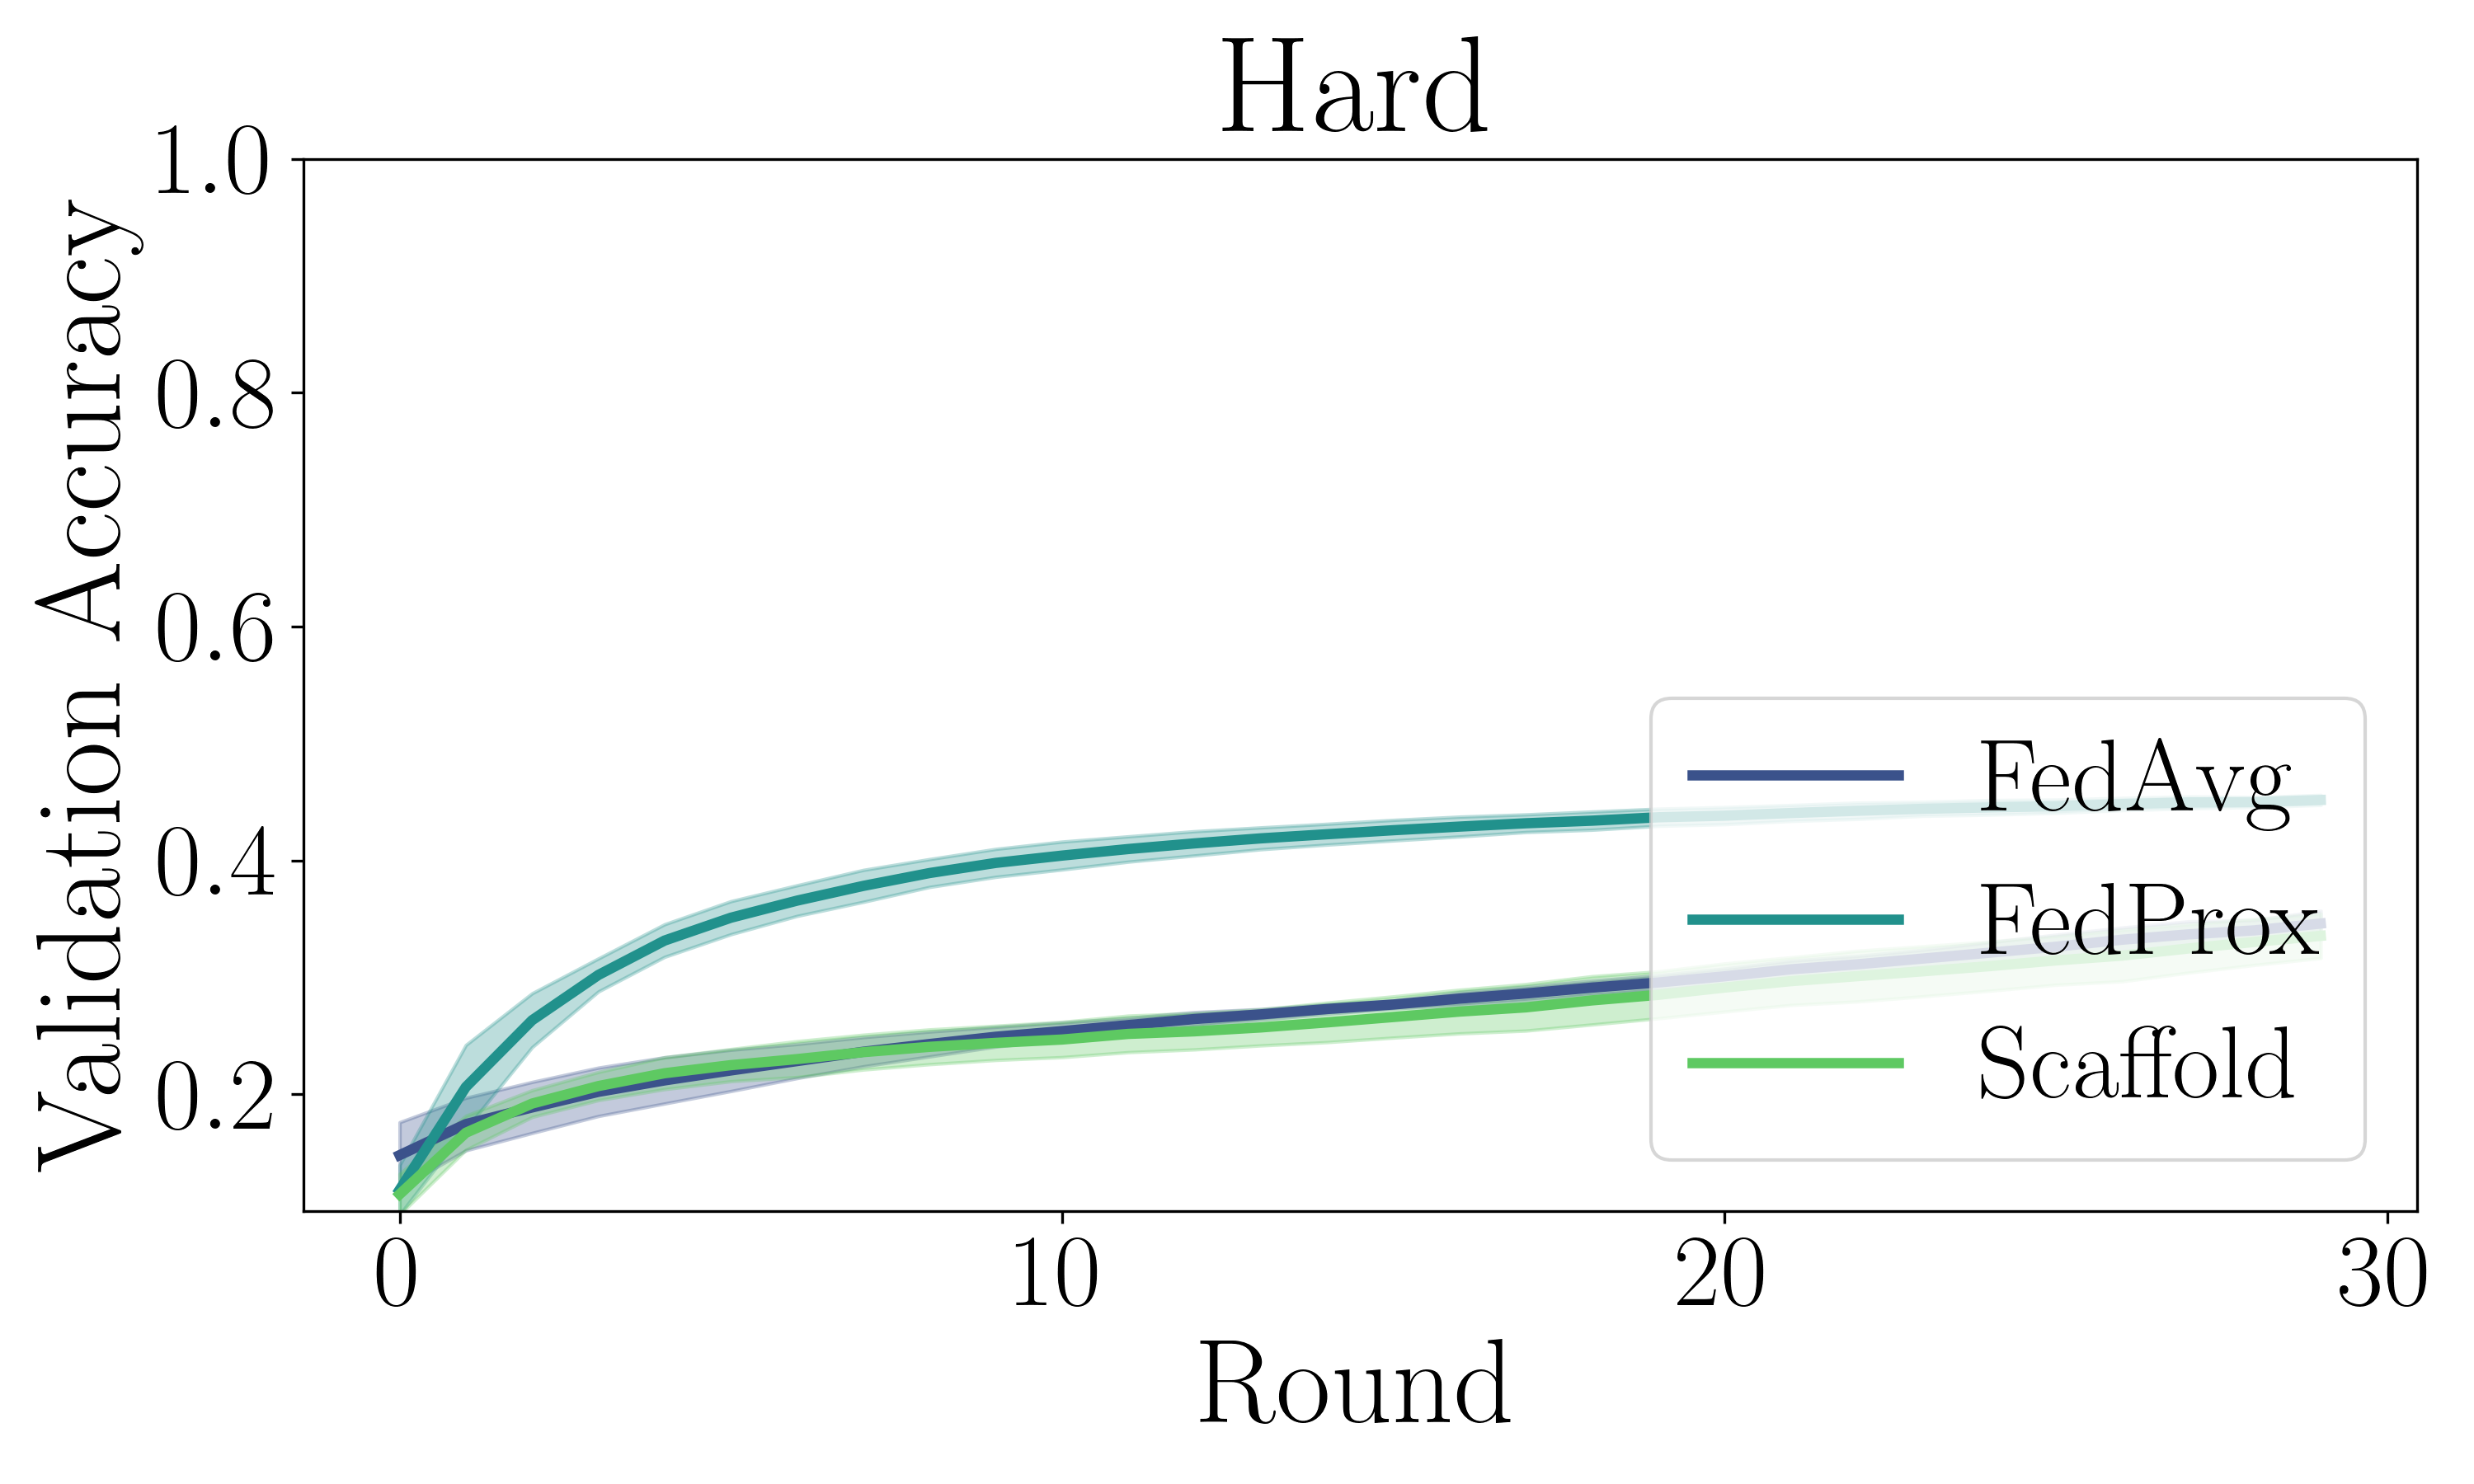
\includegraphics[width=\textwidth]{figures/ch07/profed/charts/ValidationAccuracy_dataset-EMNIST_areas-9_partitioning-Hard.png}   
    \end{subfigure}

\caption{
    Validation accuracy results across MNIST, FashionMNIST, and EMNIST datasets using Dirichlet (top row) and Hard (bottom row) partitioning methods.
}
\label{fig:exp}
\end{figure*}

